\subsection{ Cryogenic compatibility of materials for Superattenuator construction}
\label{sec:cryo_filters}

In this appendix some guide lines to select materials and components for the construction of a \emph{Superattenuator} working in a cryogenic environment are reported. Doing this it will help in the understanding process of the interface problems linked to the presence of a cryogenic payload suspended from an anti-seismic system. During our investigation, based on data coming from literature and on some lab tests performed by Virgo collaboration, no preliminary hypothesis on the operating temperature has been done keeping the maximum flexibility. Even if some construction materials (stainless steel, $OFHC$ copper, etc.) can be used down to liquid helium temperature this does not represents a limiting factor of our investigation. However, for each element of the chain, it is necessary to perform a careful characterisation test of the thermal expansion coefficient. The presence of very sophisticated optics, indeed, requests a particular attention to avoid the environment contamination that needs to be carefully controlled. The conclusions of our activity, summarised in the following, are discussed in detail in \cite{Poggiani2009}.
\begin{itemize}
\item $Actuators$: the position of different elements of the suspension system, especially those ones close to the optical payload, must be moved for the interferometer control. Some commercial stepping motors designed for Ultra High Vacuum ($UHV$) and cryogenic applications are available, but they should be tested and qualified by a dedicated characterisation measurement performed in the standard working conditions. An AML motor has been tested successfully at Virgo down to a few Kelvin [$F. Frasconi$, $Private$ $communication$]. Cryogenic lubricants should also be selected, avoiding those ones having chemical composition based on hydrocarbon and fluorine for possible contamination issues.
\item $Cabling$: the great variety of control systems and sensors in Einstein Telescope will require a large number of electrical connections, that should have low thermal conductivity (to reduce heat exchange), low electrical resistivity (to reduce dissipation), high flexibility (to reduce noise injection) and low contamination. An optimization of conductors and insulator dimensions as a function of current and operating temperature is required. As detailed in \cite{Poggiani2009}, some low out-gassing samples tested in Virgo can be used at low temperatures: Pyre-Ml insulated wires, alumina insulated wires, Gore-Tex ribbons. While $Kapton$ and $PTFE$ insulation have been already tested for satellite applications.
\item $Adhesives$: during the construction of the interferometer there will certainly be the need to bond several elements of Einstein Telescope. For this reason some adhesives could be selected and used. They must be able to withstand thermal cycling and match the thermal expansion coefficients of the bonded elements. The adhesives properties are strongly dependent on the specific batch and on the curing recipe (time and temperature). As shown in \cite{Poggiani2009} several solutions are available for testing them down to liquid helium temperature, including epoxy and ceramic adhesives. Even if some of them have been tested on optical surfaces, the bonding strength, the thermal expansion coefficient, ageing and contamination issues on long time scales must be measured by a dedicated research activity devoted to a precise characterisation of each adhesive.
\item $Magnets$: the properties of magnetic materials are strongly dependent on the temperature. Ferrite and Alnico materials are not suited below 200 K because they change magnetic properties. Neodymium-Iron-Boron magnets show an increasing magnetic field going from room temperature down to 140-120 K while decreasing its value at lower temperature. Samarium-Cobalt magnets show a magnetic field slowly decreasing with decreasing temperature and they have been successfully used down to liquid helium temperature. A critical point is the "Barkhausen noise" that we are studying in a dedicated $R\&D$ activity for a precise characterisation, as reported in the coil -magnet actuator section. 
\end{itemize}
As mentioned in the suspension chapter, another important topic deals with the creep noise of suspension elastic elements generated by the high stress applied. It has been already shown in the same section  that the noise due to the dislocations motion and to their avalanche formation are typical events triggered by the temperature increasing, important only in the last stage(s) of the \emph{Superattenuator}. The natural question is: what is the situation of this micro-glitch noise in a cryogenic environment? Even if creep is associated to an increment of the environmental temperature, cryogenic creep is not necessarily negligible, as observed for $OFHC$ copper. Data from literature on this subject and relative to steels as reported in \cite{Poggiani2010} are insufficient and scattered. Since most part of previous studies investigated transient creep, it is suggested to perform very long term tests before using this material in a cryogenic environment. In \cite{Poggiani2010} typical apparatus to measure creep in a cryogenic environment are outlined. An $R\&D$ program is required only if in the final design of Einstein Telescope some elastic elements will operate at low temperature. 

%%
%% Suspensions chapter
%%
%% Author:
%% Version:
%%
%\documentclass[color,cite,epsfig,12pt]{article}
%\usepackage{graphicx}
%\usepackage{placeins}
%\begin{document}
%%\bibliographystyle{unsrt} 



%%
%\vskip 3mm
%%
\subsection{Geometric anti-springs as seismic attenuation filters}
%%\subsection{Geometric anti-springs as seismic attenuation filters}
\label{sec:Gas_spring}
\vskip 2mm
An evolution of the Virgo mechanical filter to be used as vertical seismic noise  
suppression system, has been developed at Caltech~\cite{cella}, AEI and NIKHEF.
The anti-spring effect of this new technolgy is based on a particular geometry of the
elastic elements, the blades, mounted on a metallic disk and forming the so called 
\emph{Geometric Anti-Springs} (GAS) filter.
Seismic filters based on this effect have been successfully employed in the TAMA 
interferometer~\cite{tamaexperience} and now the GAS solution represents the baseline 
option for the optical components suspensions of the cryogenic and underground gravitational 
waves detector LCGT at Kamioka in Japan.

The GAS filter, shown in Fig.~\ref{fig:gas1}, consists of a set of radially arranged cantilever 
spring blades clamped at the base to a common frame disk and opposing each other via a central 
ring or keystone. 
\begin{figure}[htbp!]
\centering
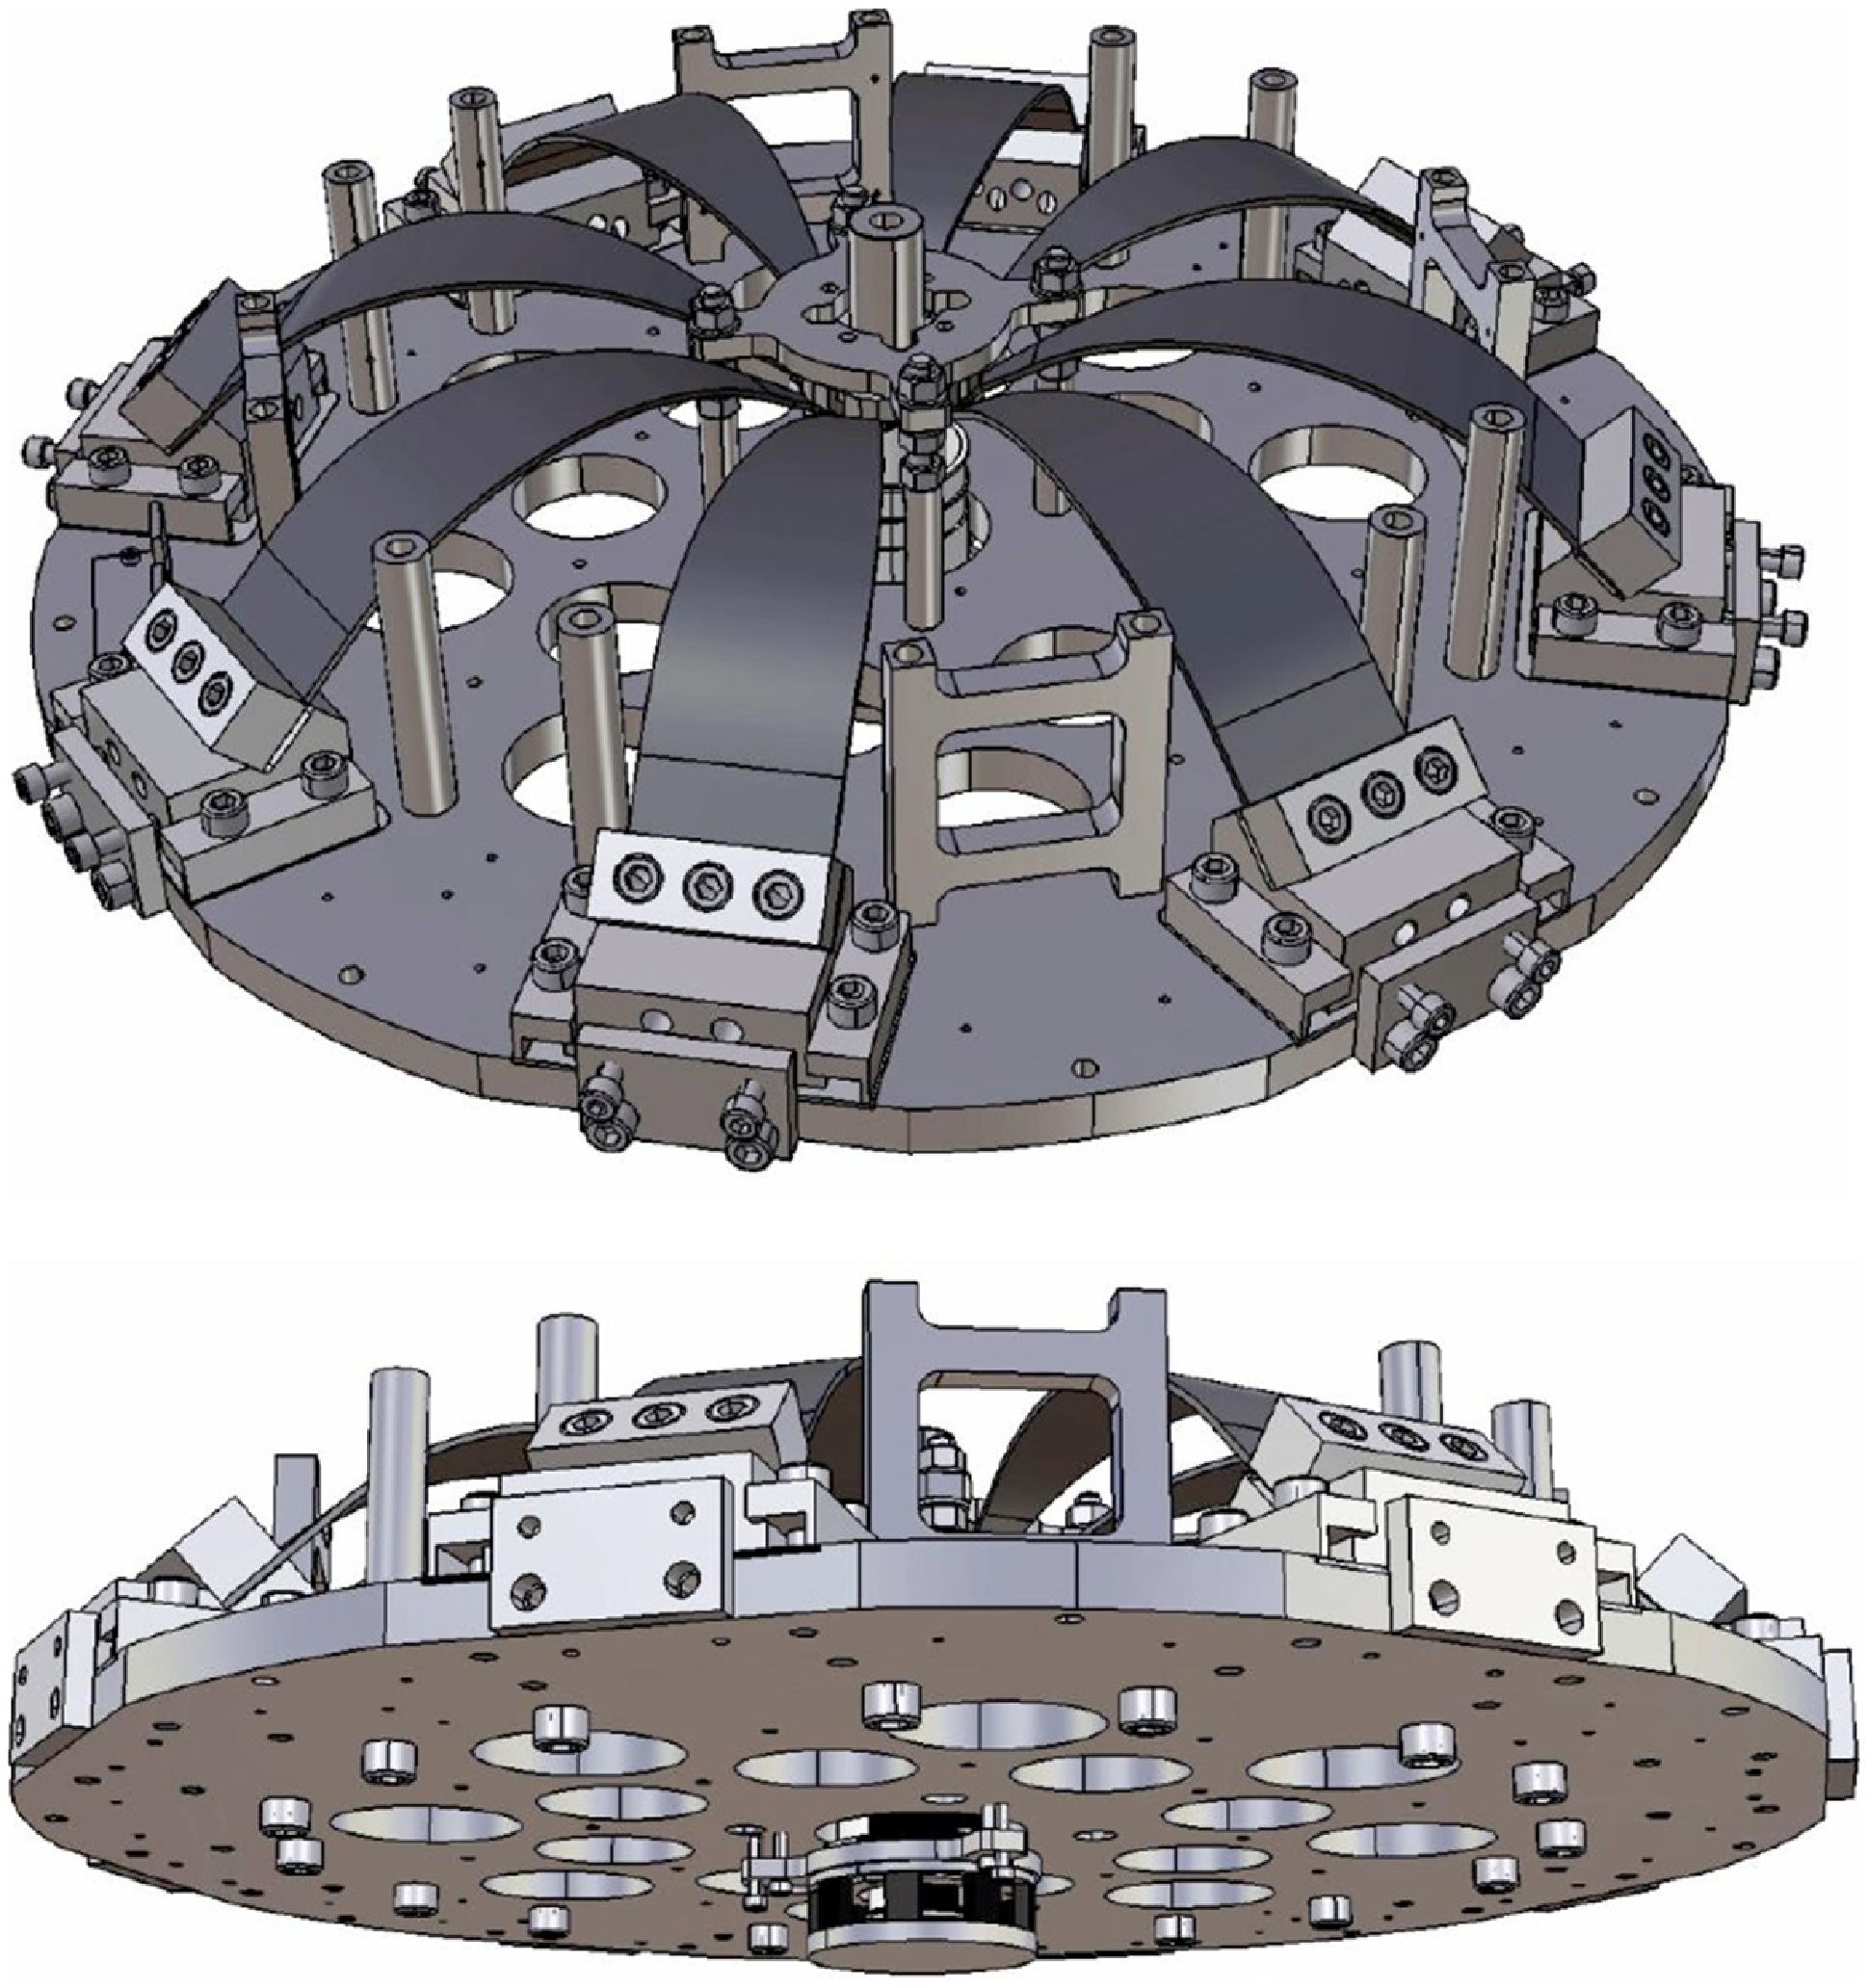
\includegraphics[width=6cm]{./Sec_Suspensions/Figures/gas1.pdf}
\caption{A 3D rendering view of a GAS filter used as seismic isolation system for the 10 m 
long interferometer at AEI Hannover. The same technology is used by the NIKHEF group for 
the the optical bench of the light injection in the interfrometer of Advanced Virgo. A voice coil actuator, visible on the bottom part of the figure, 
is located in the center of the filter.}
\label{fig:gas1}
\end{figure}

The blades are machined with a flat triangular shape while they become bended as soon as 
a suitable load is applied on their bases pushing the mechanical structure toward
the filter center. Since these elastic elements are compressed with a very high stress,
(up to 1.8 GPa) the material choice for their construction plays a fondamental role. To this 
purpose the Maraging steel ~\cite{Braccini2000} has been selected because it guarantees 
low creep noise level, low deformability and high thermal stability under high stress applied.
Each filter is an adjustable spring formed by a crown of curved cantilever blades compressed 
each against the other: the constrained radial stress creates an anti-spring effect 
(geometric anti-spring)~\cite{Bertolini} that allows a low effective stiffness to be achieved 
in the vertical direction when the nominal load is hung. 

The main features of the GAS filters are:
\begin{itemize}
\item{} Compact design with a limited number of mechanical elements;
\item{} UHV compatible;
\item{} Fast assembly and tuning;
\item{} Possibility to implement an active control (e.g.\ electro-magnetic antispring EMAS) 
with LVDT sensor and a voice coil actuator integrated into the design; 
\item{} Excellent attenuation performance when carefully tuned and operated under vacuum.
\end{itemize}

A photo of a geometric anti-spring assembled at NIKHEF and an LCGT prototype is shown 
in Fig.~\ref{fig:gas_nikhef}.

\begin{figure}[htbp!]
\centering
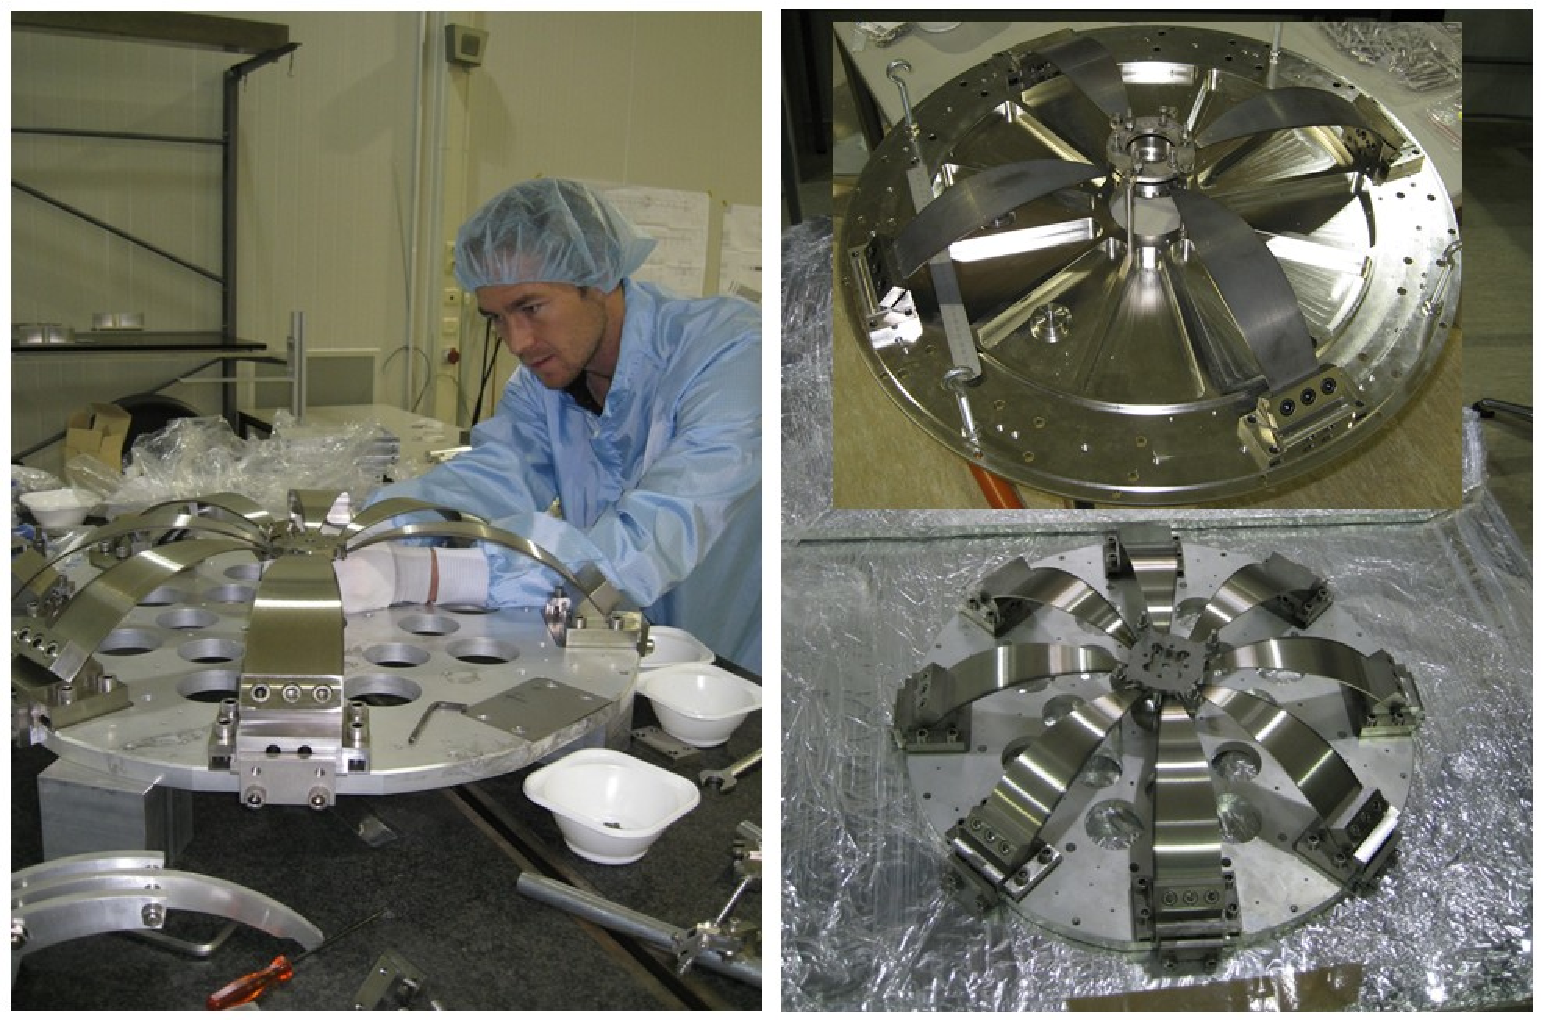
\includegraphics[width=9cm]{./Sec_Suspensions/Figures/gas_nikhef.pdf}
\caption{Pictures of the GAS filter prototypes. The left and top right panels
show a filter built and tested at NIKHEF for the Virgo external injection bench ~\cite{nikhef}.
The bottom right panel shows a prototype for LCGT suspension.}
\label{fig:gas_nikhef}
\end{figure}

A vertical cut-off frequency down to 0.30\,Hz have been obtained through a fine mechanical 
adjustment of the compression rate while longer natural period can be achieved by applying 
positive feedback (the so-called electro-magnetic anti-spring - EMAS). 
The performance of a GAS filter is shown in Fig. \ref{fig:hamsassensv} where a comparison 
between the model and the measurements performed using a system with three blades is reported.
In the plot a seismic attenuation performance of -60 dB at about 10 Hz is visible
while an isolation level down to -80 dB (at frequncy higher than 10 Hz) can be reached by using 
a set of overcompensating wands ~\cite{stochino}.

\begin{figure}[htbp!]
\centering
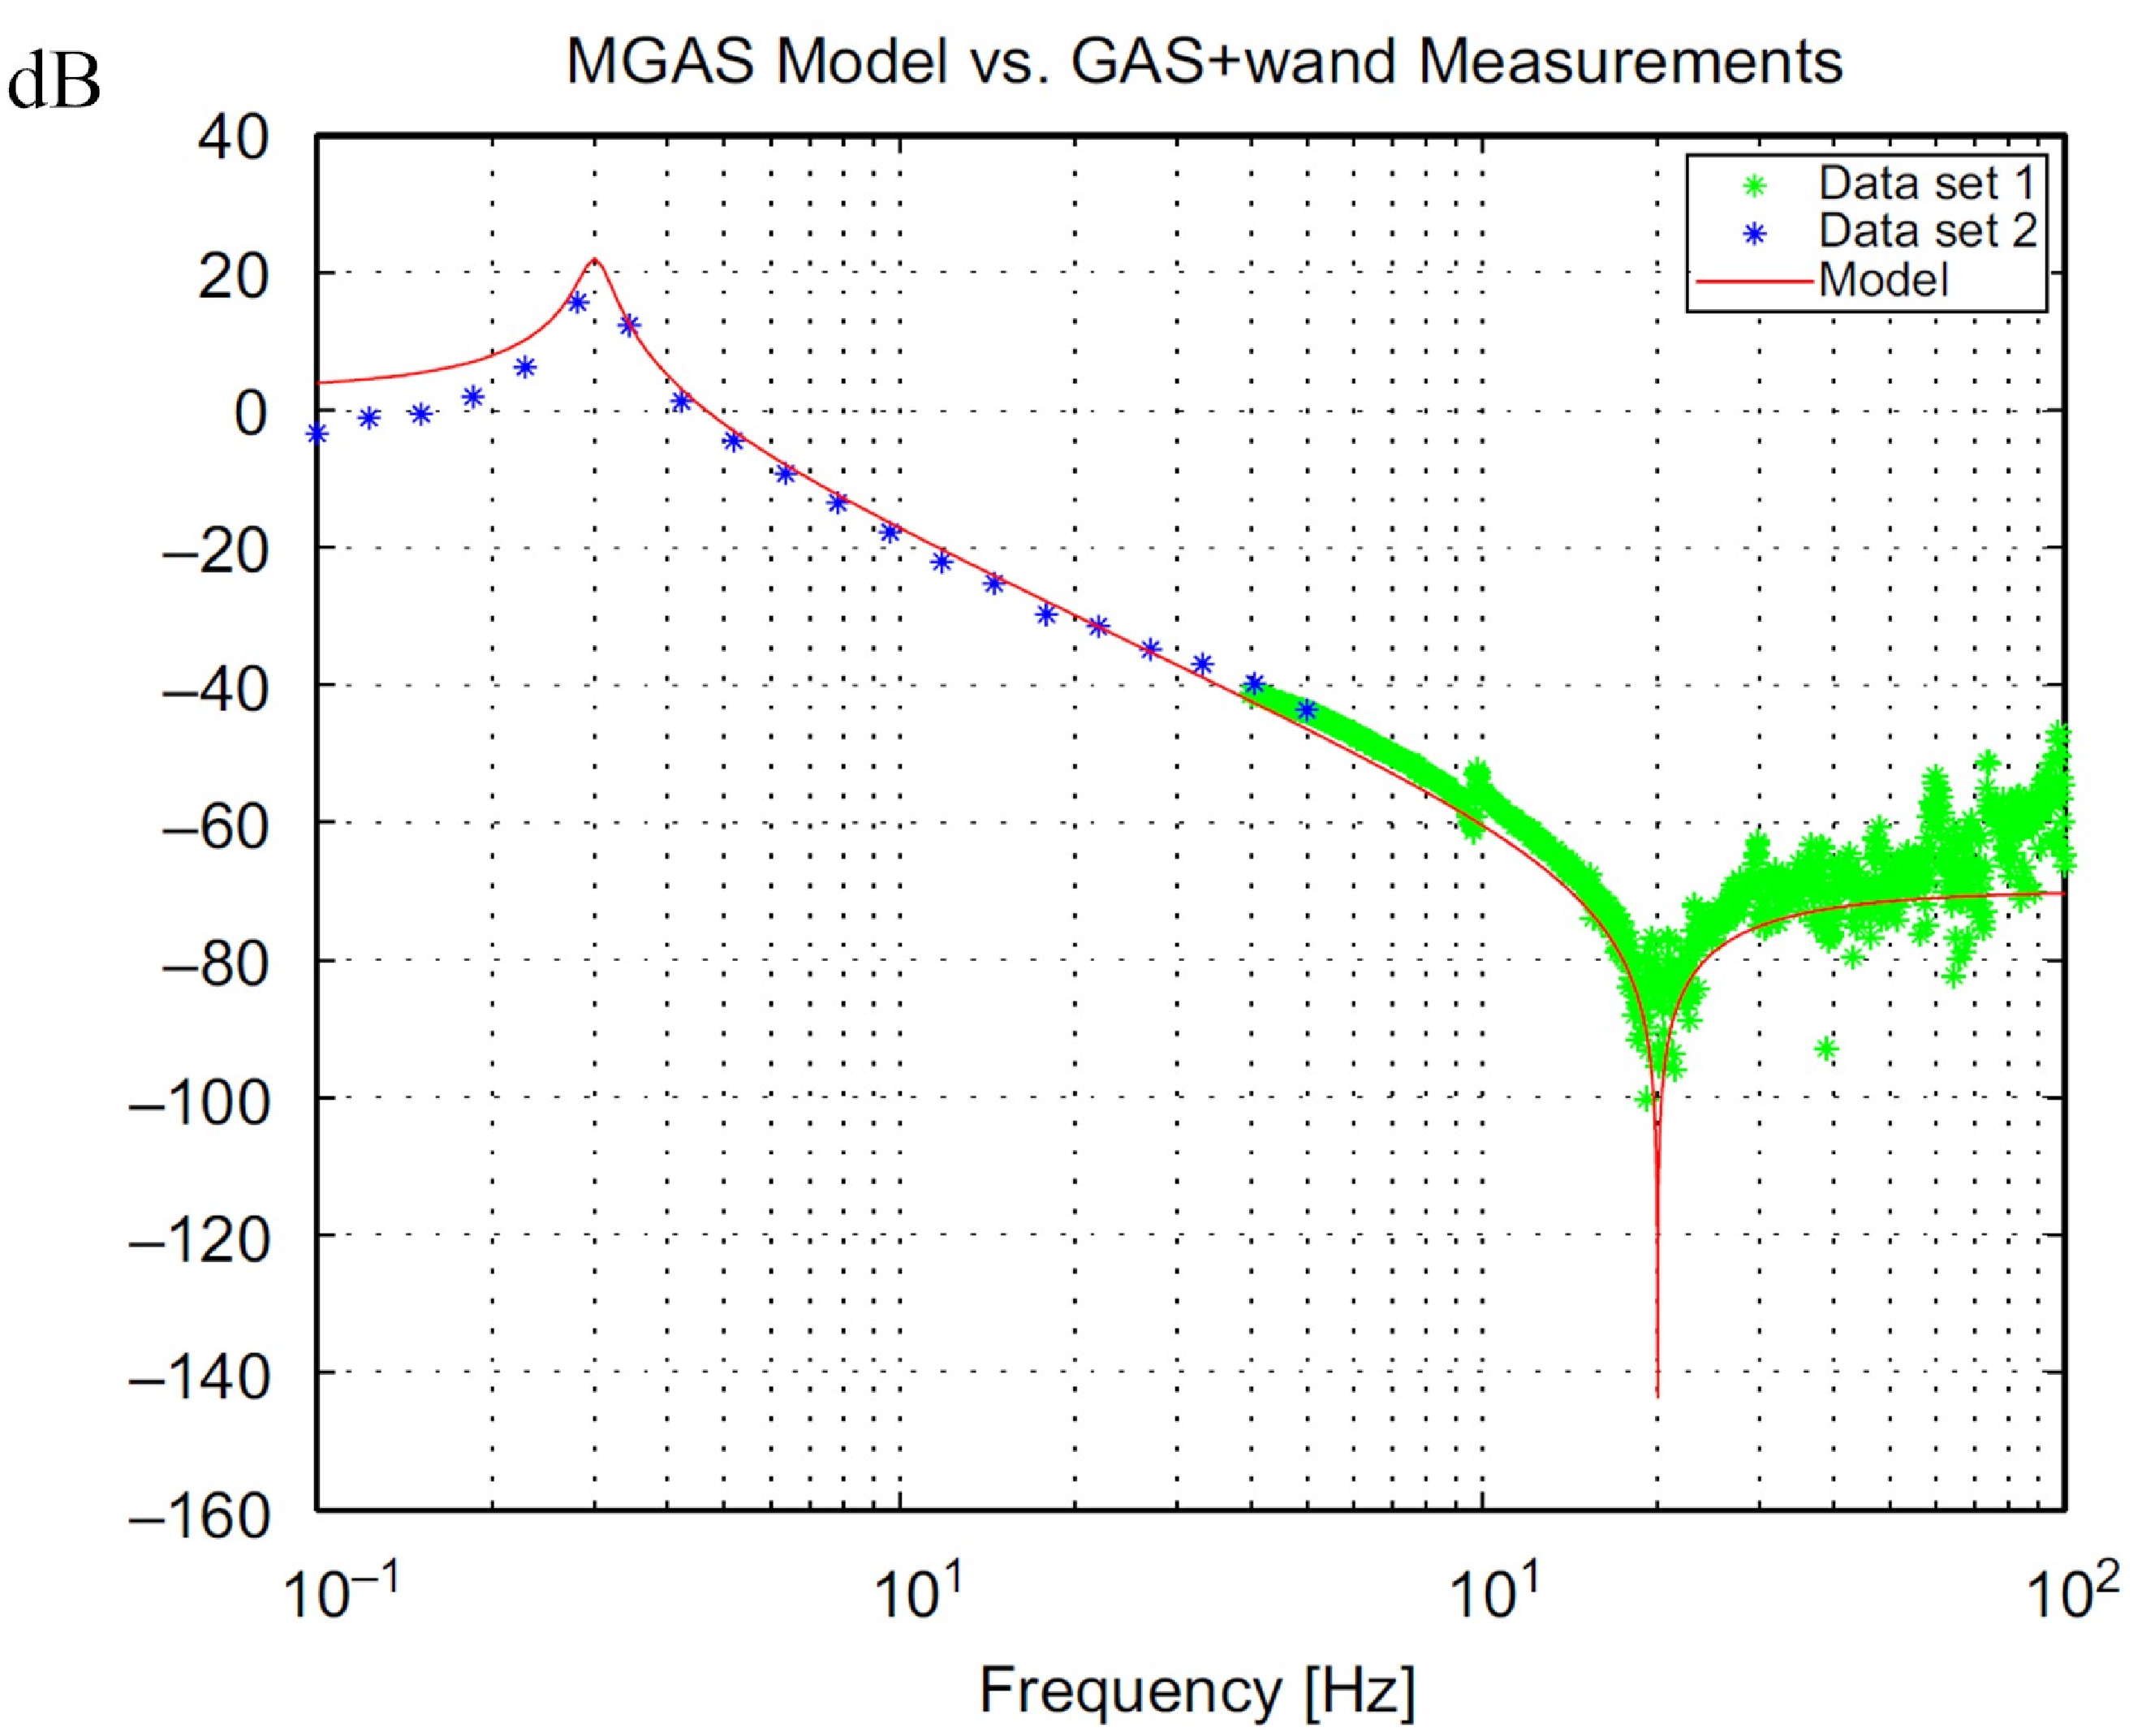
\includegraphics[width=10cm]{./Sec_Suspensions/Figures/hamsassensv.pdf}
\caption{Vertical attenuation performance of a GAS filter with overcompensating 
wands \cite{stochino}}
\label{fig:hamsassensv}
\end{figure}

Finite element analysis (FEA)~\cite{Hennes} and a measurements campaign on a GAS filter 
prototype are in progress in AEI Hannover and NIKHEF. They provide valuable input 
for the GAS filter fine tuning and its behaviour as a function of the environmental temperature.  
Detailed studies on a filter prototype for LCGT project and with different blades shapes 
are also in progress at NIKHEF.
 

%\end{document}
%%
%% Suspensions chapter
%%
%% Author:
%% Version:
%%
%\documentclass[color,cite,epsfig,12pt]{article}
%\usepackage{graphicx}
%\usepackage{placeins}

%\begin{document}
%%\bibliographystyle{unsrt} 

\subsection{The LIGO active seismic filters}
%%\subsection{The LIGO active seismic filters}
\label{sec:LIGO_filters}

%\emph{Author:  F. Ricci}

In the the Advanced LIGO project the seismic noise suppression problem has been fixed using
a different approach \cite{aLIGO}. The suspension chain has been designed including 
an in-vacuum two-stage active isolation system where the inner modes are reduced by sensing 
the stage motion and applying forces in feedback loops. 

The in-vacuum attenuator provides isolation above about 0.2 Hz and consists of two-stages 
platforms connected to each other by springs. Each stage is supported by three maraging 
steel blade springs and short pendulums from the stage above it to provide vertical and 
horizontal compliance in six degrees of freedom (see fig. \ref{fig:active_filter} left side). 
Contained in each stage are six position sensors and six seismometers which collectively measure 
motion in all degrees of freedom. The signals from these detectors are feed-back to magnetic 
actuators to reduce the motion of the platforms. The rigid body modes of these stages are 
between 1.3 and 7 Hz, while the unity gain frequency of the control loop will be at about 25 Hz. 
Together, these stages provide isolation of about a factor of 300 at 1 Hz and about 3000 at 10 Hz, 
in amplitude. The second stage contains an optical table, from which the suspension and test 
mass are supported.

\begin{figure}[htbp!]
\centering
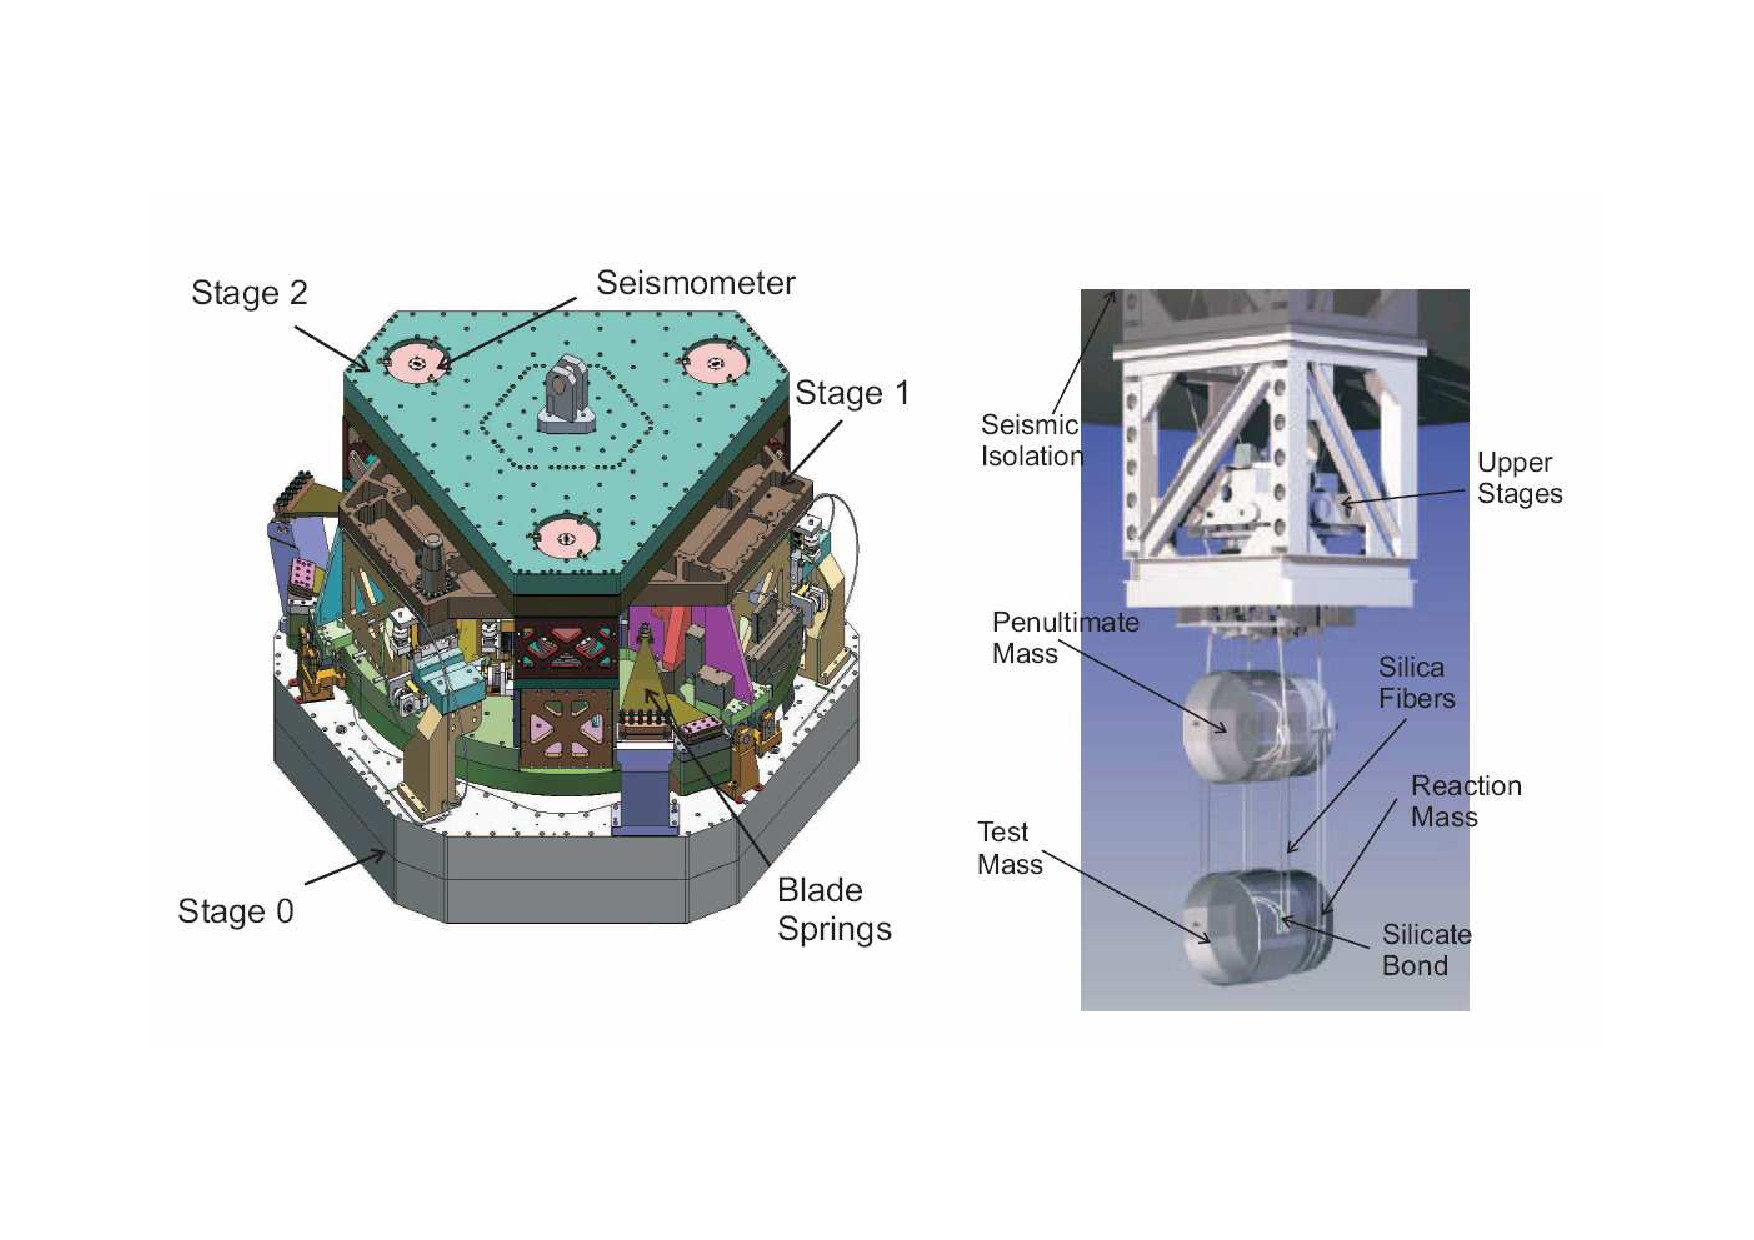
\includegraphics[width=14cm]{./Sec_Suspensions/Figures/Active_filter_2.pdf}
\caption{Internal stages of the large vacuum chamber seismic isolation system (left side).
Advanced LIGO suspension: the test mass connected at the bottom to the penultimate mass above
it with silica fibers. On right side, the reaction mass behind the test mass is visible}
\label{fig:active_filter}
\end{figure}

The Advanced LIGO test masses will be supported by suspensions that hang below the seismic
isolation platforms. These suspensions are multistage pendulums with a final stage consisting
of the test mass hanging on fused silica fibers. They will provide additional passive isolation,
allow for necessary control forces to be applied without adding excess noise, and minimize the
effect of thermal noise.

In addition to the main quadruple suspension chain that supports the test mass, there will also
be a nearly identical reaction chain placed 5 mm behind it (see fig. \ref{fig:active_filter} 
right side). This chain will allow control forces for global angular and longitudinal degrees 
of freedom to be applied from a quiet platform. These forces will be hierarchically used, 
with large forces applied with coils and magnets between both the upper intermediate and 
penultimate masses but with fine control forces applied with an electrostatic drive (ESD). 
The ESD is a gold pattern deposited on the face of the final reaction mass and applies 
forces to the test mass with an electrostatic field.
Local damping of all the low frequency suspension modes will be done with co-located sensors
and actuators on the top mass to insure that any sensing noise will be well isolated from the
test mass.

\noindent
The main feature of this suspension, shorter than the Virgo Superattenuator, is represented by 
the fact that the final isolation requirements are reached with a system based mainly on an 
active hierarchical control.


%\end{document}




